\providecommand{\main}{..}		% Override relative path to the main file (already set in main file)
\documentclass[../InterneDSLs.tex]{subfiles}
\begin{document}

\chapter{Bau des Prototypen}\label{SEC:Prototype}

\section{Aufbau}
Die Verarbeitung der Grammatik erfolgt nach dem folgenden Schema:
\begin{itemize}
	\item Parsen der Grammatik
	\item Aufbau des Syntax-Baumes
	\item Abbildung in einen Graphen, der die Aufrufreihenfolge abbildet
	\item Generierung der Interfaces mit StringTemplates
\end{itemize}

\section{Parsen der Grammatik}
Für das Parsen der Grammatik wurde ANTLR4 verwendet, der adaptive LL(*)-Parser generieren kann, die Grammatiken zur Laufzeit analysieren können, statt zur Compilezeit (siehe~\cite[S. xiii ff]{Parr.2012}). ANTLR selbst ist in Java geschrieben und kann Parser für verschiedene Zielsprachen generieren (u.a. Java, C++, C\#, Python, vgl.~\ref{antlrcodegeneration.github}). Da neue Features vorrangig für den Parser in Java entwickelt werden, und da als Zielsprachen JVM-Sprachen ins Auge gefasst wurden, wird auf dem Parser in Java aufgebaut werden.

Um die Grammatiken zu notieren verwendet ANTLR eine Syntax die sich nicht an der ISO-Norm sondern an einer alten EBNF-Variante orientiert. In dieser Syntax wurde eine Grammatik erstellt, um die in Abschnitt~\ref{SEC:SetSyntax} festgelegte Notation der EBNF zu parsen (Listing~\ref{LST:EBNFGrammar}). Beim verfassen der Grammatik wurde schon darauf Rücksicht genommen, dass man Schlüsselworte und Typen (einer Programmierspraceh) angeben kann (siehe Listing~\ref{LST:EBNFGrammar} Zeile 24-33).

\begin{figure}[ht]
\lstinputlisting[linerange={3-35},caption={EBNF-Grammatik (Auszug)},label={LST:EBNFGrammar}]{Bnf.g4}
\end{figure}

Um den Parse-Tree der eingelesenen Grammatik zu verarbeiten, bietet ANTLR4 zwei Möglichkeiten: generierte Listener oder Visitor zu überschreiben (vgl.~\cite[S. 112 ff]{Parr.2012}). Die Visitors sollte man implementieren, falls man größtmögliche Kontrolle über das traversieren des Baumes benötigt. Da das aber nicht nötig ist, werden hier nur die Listener erweitert, um aus den EBNF-Konstrukten (die praktisch Strings entprechen) einen Baum aus eigenen Klassen generiert. Dadurch wird eine Typ-Sicherheit hergestellt, die durch die Strings im EBNF-Parser selbst nicht gegeben ist.

Abbildung~\ref{FIG:TypesBNF} zeigt die eigenen Typen des Baumes, der dem Parse-Tree entspricht; in ihm finden sich die Konstrukte der EBNF wieder (z.B. Regeln, Sequenzen, Alternativen, vgl. Abbildung~\ref{LST:EBNFGrammar}). Aus dem Baum dieser Typen werden die Interfaces generiert, wie im folgenden Abschnitt~\ref{SEC:EBNFtoInterface} erklärt wird.

\begin{figure}[ht]
\centering
\includegraphics[width=\linewidth]{\main/10_Pictures/BNF-Types}
\caption{Typen des BNF-Baumes}
\label{FIG:TypesBNF}
\end{figure}

\section{Abbildung von EBNF auf Interfaces}\label{SEC:EBNFtoInterface}
Aus dem Baum ein Graph generiert, dessen Abfolge von Knoten und Kanten die Konstrukte der EBNF darstellt. Die Knoten werden dabei dazu verwendet, die Scopes für das Object Scoping zu repräsentieren, der Typ und die Anzahl der Kanten repräsentierten die Konstrukte der EBNF selbt. Wie die Konstrukte genau abgebildet werden, wird in den folgenden Abschnitten erklärt. Neben den trivialen Fällen wird auf einige verschachtelte Konstrukte eingegangen um zu zeigen, dass einige Konstrukte im Graph verwendet werden, die aus den trivialen Fällen nicht ersichtlich sind.

Zuerst werden jedoch die Eigenschaften des Graphen erläutert und dazu eine entsprechende Bibliothek ausgewählt.

\subsection{Eigenschaften des Graphen}
Aus der Struktur der EBNF gehen verschiedene Eigenschaften des Graphen heraus; er Graph ist
\begin{itemize}
	\item gerichtet (wegen der Sequenz),
	\item zyklisch (Wiederholung),
	\item ungewichtet (keine Alternative wird bevorzugt) und
	\item kann parallele Kanten enthalten (Alternative).
\end{itemize}
Diese Eigenschaften bezeichnen einen gerichteten, zyklischen Multi- bzw. Pseudograph. Die parallelen Kanten haben eine eigene Identität (Name und Typ), mit der man sie von anderen Kanten mit dem selben Quell- und Zielknoten unterscheiden kann.

Da es bei allen im folgenden vorgestellten Abbildungen jeweils einen Knoten ohne eingehende Kanten und einen Knoten ohne ausgehende Kanten gibt, hat der gesamte Graph ebenfalls einen Start- und End-Knoten. Dadurch sind der Start und das Ende des Graphen gegeben, was das Traversieren vereinfacht, der Endknoten kann ebenfalls einfach für eine Build-Methode identifiziert werden.

Beide Start- und End-Knoten müssen im Graph-Builder jedoch manuell verfolgt werden, da während dem Aufbau des Graphen (etwa bei der Alternative) mehrere Knoten mit den Eigenschaften des Endknoten auftreten können.

\subsubsection{Graphbibliotheken}
Es gibt mehrere bekannte Bibliotheken für Graphen in Java, die sich im Umfang und Status der Weiterentwicklung unterscheiden. Auf eine Eigenentwicklung wird verzichtet, da die Graphen und zugehörigen Algorithmen in den Bibliotheken schon getestet sind. Hier werden drei Bibliotheken vorgestellt, von denen JGraphT ausgewählt wurde, da hier der Fokus auf die Graphen und Algorithmen gelegt wurde.
\begin{itemize}
	\item JGraphT\footnote{\url{https://jgrapht.org/}}
	\item Google Guava\footnote{\url{https://github.com/google/guava}}
	\item Apache Commons\footnote{\url{https://commons.apache.org/sandbox/commons-graph/}}
\end{itemize}

\paragraph{JGraphT}
JGraphT wird aktiv weiterentwickelt und bietet Typen für verschiedene Arten von Graphen (u.a. gerichtete/ungerichtete, gewichtet/ungewichtet)~\cite{JGraphT}. Außerdem bietet die diese Bibliothek die Möglichkeit eigene Typen für Knoten und Kanten anzugeben, womit man für beide jeweils Identitäten vergeben kann (z.B. spezielle Namen für den Start- und End-Knoten). Darüber hinaus implementiert JGraphT für Graphen typische Algorithmen (u.a. Shortest Path, Coloring, Tiefensuche, Breitensuche, Zyklenerkennung) und Exportfunktionen (z.B. DOT).

Es gibt auch Adapter, um die Algorithmen von JGraphT auf die Typen von Google Guava anzuwenden.

\paragraph{Google Guava}
Google Guava beinhaltet unter anderem auch Typen für Graphen, mit benutzerdefinierten Typen für Knoten oder Knoten und Kanten. Auch gerichtete/ungerichtete und gewichtete/ungewichtete Graphen sind möglich. Aber es gibt kaum Algorithmen, die auf den Typen arbeiten.

\paragraph{Apache Commons}
Apache Commons bietet auch eine Graph-Bibliothek, die (un)gerichtete und (un)gewichtete Graphen erlaubt, wenige Algorithmen bietet aber nicht mehr weiterentwickelt wird und nur als Version 0.1 vorliegt.

\subsubsection{Typen}
Abbildung~\ref{FIG:GraphTypes} zeigt die eigenen Typen des Graphen: die Scopes werden als Knoten verwendet und die ScopeEdges als Kanten. Erstere repräsentieren die Interfaces, die letzteren, je nach Klasse und Typ eine Vererbungsbeziehung oder Methode inklusive Argumente.

OptionalEdges repräsentieren eine Vererbungsbeziehung, deswegen darf es zwischen zwei Knoten nur eine OptionalEdge geben; eine OptionalEdge mit demselben Quell- und Zielknoten ist ebenfalls nicht erlaubt, da diese Kante überflüssig ist.

NodeEdges mit dem Typ \gqq{KEYWORD} werden zum Schlüsselwort der generierten Sprache, indem für sie eine Methode generiert werden, die den Bezeichner aus der EBNF als Methodennamen verwendet (weitergereicht als String im Node in Abbildung~\ref{FIG:GraphTypes}). Folgt solch einer NodeEdge eine vom Typ \gqq{Type}, wird diese zu einem Argument vom in der EBNF angegebenen Typen; der Name des Typs wird automatisch generiert.

NodeEdges vom Typ \gqq{NON\_TERMINAL} entsprechen Nicht-Terminalen in der EBNF und werden benötigt, um die Nicht-Terminalen durch die entsprechenden Regeln zu ersetzen. Dazu wird für jede Regel der EBNF ein eigener Graph aufgebaut und anschließend die Nicht-Terminalen Kanten durch deren entsprechenden Graphen ersetzt.
\begin{figure}[ht]
\centering
\includegraphics[width=.85\textwidth]{Nodes}
\caption{Typen des Graphen (Scope für die Vertices; ScopeEdge, OptionalEdge und NodeEdge für die Kanten)}
\label{FIG:GraphTypes}
\end{figure}

\subsection{Kante mit einem Knoten}
Der einfachste Fall ist der von einer Sequenz, die nur ein Element beinhaltet. Hier kann das Element auf eine Kante zwischen zwei Knoten abgebildet werden. Die Namen der Scopes werden zu den Interfaces, bzw. zum Rückgabewert der Methode, deren Namen dem der der Kante entspricht. Grafik~\ref{FIG:OneElementNode} zeigt, wie eine Abbildung aussehen kann.
\begin{figure}[ht]
\centering
  \begin{subfigure}[c]{0.49\textwidth}
  	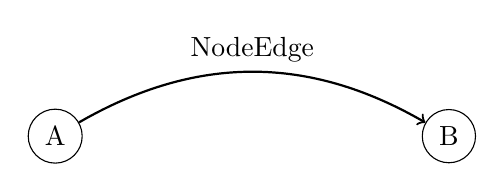
\begin{tikzpicture}
		\tikzset{vertex/.style = {shape=circle,draw,minimum size=.2em}}
		\tikzset{edge/.style = {->,> = latex'}}
		\node[vertex] (a) at  (0,0) {A};
		\node[vertex] (b) at  (5,0) {B};
		\path[->,draw,thick,bend left] (a) edge node[above] {NodeEdge} (b);
	\end{tikzpicture}
    \caption{Diagramm eines Sequenz-Knotens}
    \label{FIG:DiagramOneElementNode}
  \end{subfigure}
  \begin{subfigure}[c]{0.49\textwidth}
    \lstinputlisting[language=Java,caption={Java-Interface aus einem Sequenz-Knoten},label={LST:JInterfaceOneElementNode}]{Scope_one-element.java}
  \end{subfigure}
  \caption{Diagramm und Interface eines Sequenz-Knotens (\texttt{<rule> = NodeEdge;})}
  \label{FIG:OneElementNode}
\end{figure}

\subsection{Sequenz von Knoten}
Tritt eine Sequenz von Knoten auf, muss für jeden Knoten ein Interface mit einer Methode generiert werden, um die Aufruf-Reihenfolge zu gewährleisten. Abbildung~\ref{FIG:SequenceNode} zeigt ein Beispiel mit zwei Knoten in einer Sequenz.
\begin{figure}[ht]
\centering
  \begin{subfigure}[c]{0.49\textwidth}
  	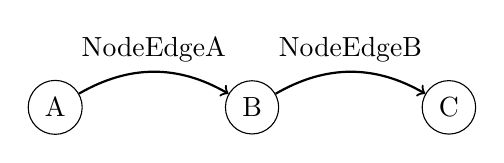
\begin{tikzpicture}
		\tikzset{vertex/.style = {shape=circle,draw,minimum size=.2em}}
		\tikzset{edge/.style = {->,> = latex'}}
		\node[vertex] (a) at  (0,0) {A};
		\node[vertex] (b) at  (2.5,0) {B};
		\node[vertex] (c) at  (5,0) {C};
		\path[->,draw,thick,bend left] (a) edge node[above] {NodeEdgeA} (b);
		\path[->,draw,thick,bend left] (b) edge node[above] {NodeEdgeB} (c);
	\end{tikzpicture}
    \caption{Diagramm einer Sequenz von Knoten}
    \label{FIG:DiagramSequenceNode}
  \end{subfigure}
  \begin{subfigure}[c]{0.49\textwidth}
    \lstinputlisting[language=Java,caption={Java-Interfaces aus einer Sequenz von Knoten},label={FIG:JInterfaceSequenceNode}]{Scope_sequence.java}
  \end{subfigure}
  \caption{Diagramm und Interface einer Sequenz von Knoten (\texttt{<rule> = NodeEdgeA NodeEdgeB;})}
  \label{FIG:SequenceNode}
\end{figure}

\subsection{Kante mit Alternativen}
Alternativen in der EBNF können auf zwei Kanten von einem zu zwei verschiedenen Knoten abgebildet werden (siehe Abbildung~\ref{FIG:DiagramAlternativeNodeVariant}). Bei dieser Variante erhält jede Alternative einen eigenen End-Knoten. Das hat jedoch den Nachteil, dass wenn der Alternative in einer Sequenz weiter Elemente folgen, diese auf allen Pfaden der jeweiligen Alternativen dupliziert werden müssen.
\begin{figure}[ht]
\centering
  \begin{subfigure}[c]{0.49\textwidth}
  	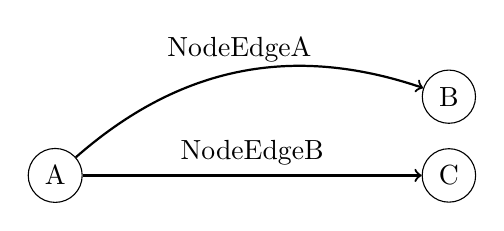
\begin{tikzpicture}
		\tikzset{vertex/.style = {shape=circle,draw,minimum size=.2em}}
		\tikzset{edge/.style = {->,> = latex'}}
		\node[vertex] (a) at  (0,0) {A};
		\node[vertex] (b) at  (5,1) {B};
		\node[vertex] (c) at  (5,0) {C};
		\path[->,draw,thick, bend left] (a) edge node[above] {NodeEdgeA} (b);
		\path[->,draw,thick] (a) edge node[above] {NodeEdgeB} (c);
	\end{tikzpicture}
    \caption{Diagramm alternativer Kanten}
    \label{FIG:DiagramAlternativeNodeVariant}
  \end{subfigure}
  \begin{subfigure}[c]{0.49\textwidth}
    \lstinputlisting[language=Java,caption={Java-Interface aus alternativen Kanten},label={LST:JInterfaceAlternativeNodeVariant}]{Scope_alternative_variant.java}
  \end{subfigure}
  \caption{Diagramm und Interface alternativer Kanten (\texttt{<rule> = NodeEdgeA | NodeEdgeB;})}
  \label{FIG:AlternativeNodeVariant}
\end{figure}

Deshalb werden stattdessen die Alternativen auf parallele Kanten zwischen zwei Knoten abgebildet (siehe Abbildung~ref{FIG:DiagramAlternativeNode}). Dadurch können die Alternativen jeweils wie Sequenzen zwischen dem selben Start- und End-Knoten abgebildet werden.
\begin{figure}[ht]
\centering
  \begin{subfigure}[c]{0.49\textwidth}
  	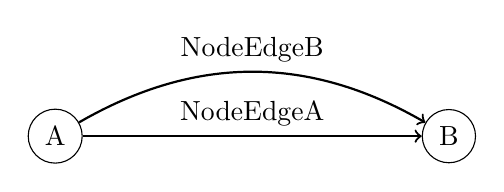
\begin{tikzpicture}
		\tikzset{vertex/.style = {shape=circle,draw,minimum size=.2em}}
		\tikzset{edge/.style = {->,> = latex'}}
		\node[vertex] (a) at  (0,0) {A};
		\node[vertex] (b) at  (5,0) {B};
		\path[->,draw,thick] (a) edge node[above] {NodeEdgeA} (b);
		\path[->,draw,thick, bend left] (a) edge node[above] {NodeEdgeB} (b);
	\end{tikzpicture}
    \caption{Diagramm alternativer Kanten}
    \label{FIG:DiagramAlternativeNode}
  \end{subfigure}
  \begin{subfigure}[c]{0.49\textwidth}
    \lstinputlisting[language=Java,caption={Java-Interface aus alternativen Kanten},label={LST:JInterfaceAlternativeNode}]{Scope_alternative.java}
  \end{subfigure}
  \caption{Diagramm und Interface alternativer Kanten (\texttt{<rule> = NodeEdgeA | NodeEdgeB;})}
  \label{FIG:AlternativeNode}
\end{figure}

\subsection{Optionales Element}
Im Falle eines optionalen Elementes, muss auch der Methodenaufruf optional sein und auch der nächstfolgende Methodenaufruf verfügbar sein. Das wird dadurch erreicht, indem das erste Interface vom folgenden erbt. Im Graphen wird das durch eine parallele Kante eines anderen Typen (OptionalEdge in Abbildung~\ref{FIG:DiagramOptionalNode}) repräsentiert. Listing~\ref{LST:JInterfaceOptionalNode}) ist, bis auf die Vererbung, gleich zu Listing~\ref{LST:JInterfaceOneElementNode}.
\begin{figure}[ht]
\centering
  \begin{subfigure}[c]{0.49\textwidth}
  	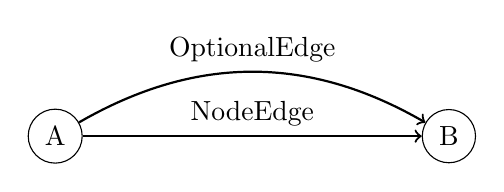
\begin{tikzpicture}
		\tikzset{vertex/.style = {shape=circle,draw,minimum size=.2em}}
		\tikzset{edge/.style = {->,> = latex'}}
		\node[vertex] (a) at  (0,0) {A};
		\node[vertex] (b) at  (5,0) {B};
		\path[->,draw,thick] (a) edge node[above] {NodeEdge} (b);
		\path[->,draw,thick, bend left] (a) edge node[above] {OptionalEdge} (b);
	\end{tikzpicture}
    \caption{Diagramm einer optionalen Kante}
    \label{FIG:DiagramOptionalNode}
  \end{subfigure}
  \begin{subfigure}[c]{0.49\textwidth}
    \lstinputlisting[language=Java,caption={Java-Interface aus einer optionalen Kante},label={LST:JInterfaceOptionalNode}]{Scope_optional.java}
  \end{subfigure}
  \caption{Diagramm und Interface einer optionalen Kante (\texttt{<rule> = [NodeEdgeA];})}
  \label{FIG:OptionalNode}
\end{figure}

\subsection{Kante mit optionaler Schleife}
Da die Wiederholung bei EBNF optional ist (beliebig oft oder keinmal auftreten darf), gibt es hier, wie beim optionalen Element eine Kante vom Typ OptionalEdge. Dadurch kann der Methodenaufruf übersprungen werden.

Um den Methodenaufruf wiederholbar zu machen kann man nicht einfach eine parallele, optionale Kante in die entgegengesetzte Richtung einfügen, weil diese ebenfalls in eine Vererbung umgesetzt würde; dadurch würde zwischen beiden Interfaces eine zirkuläre Abhängigkeit entstehen, die in Java verboten ist.

Stattdessen wird bei der optionalen Wiederholung die Kante, die den Methodenaufruf repräsentiert, eine Schleife zum Knoten selbst. Somit kann die Methode beliebig oft aufgerufen werden, bevor die in B deklarierte Methode aufgerufen wird (Abbildung~\ref{FIG:DiagramLoopNode}).
\begin{figure}[ht]
\centering
  \begin{subfigure}[c]{0.49\textwidth}
  	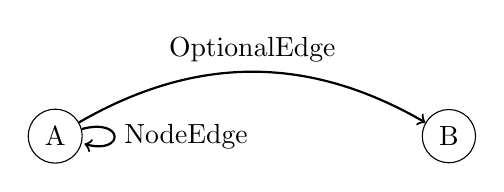
\begin{tikzpicture}
		\tikzset{vertex/.style = {shape=circle,draw,minimum size=.2em}}
		\tikzset{edge/.style = {->,> = latex'}}
		\node[vertex] (a) at  (0,0) {A};
		\node[vertex] (b) at  (5,0) {B};
		\path[->,draw,thick, bend left] (a) edge node[above] {OptionalEdge} (b);
		\path[->,draw,thick, loop right] (a) edge node[right] {NodeEdge} (a);
	\end{tikzpicture}
    \caption{Diagramm einer Schleifen-Kante (Variante 1)}
    \label{FIG:DiagramLoopNode}
  \end{subfigure}
  \begin{subfigure}[c]{0.49\textwidth}
    \lstinputlisting[language=Java,caption={Java-Interface aus einer Schleifen-Kante (Variante 1)},label={LST:JInterfaceLoopNode}]{Scope_loop.java}
  \end{subfigure}
  \caption{Diagramm und Interface einer Schleifen-Kante (Variante 1) (\texttt{<rule> = \{NodeEdge\};})}
  \label{FIG:LoopNode}
\end{figure}

Eine zweite Variante benötigt einen Hilfsknoten (Knoten B in Abbildung~\ref{FIG:DiagramLoopNodeAlt}). Im trivialen Fall ist dieser Hilfskonten unnötig, befindet sich die Schleife innerhalb einer Alternative sichert er aber die Wiederholung der richtigen Kante(n) (siehe Abbildung~\ref{FIG:LoopInAlternative}).
\begin{figure}[ht]
\centering
  \begin{subfigure}[c]{0.49\textwidth}
  	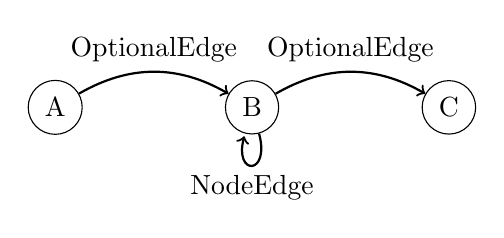
\begin{tikzpicture}
		\tikzset{vertex/.style = {shape=circle,draw,minimum size=.2em}}
		\tikzset{edge/.style = {->,> = latex'}}
		\node[vertex] (a) at  (0,0) {A};
		\node[vertex] (b) at  (2.5,0) {B};
		\node[vertex] (c) at  (5,0) {C};
		\path[->,draw,thick, bend left] (a) edge node[above] {OptionalEdge} (b);
		\path[->,draw,thick, loop below] (b) edge node[below] {NodeEdge} (b);
		\path[->,draw,thick, bend left] (b) edge node[above] {OptionalEdge} (c);
	\end{tikzpicture}
    \caption{Diagramm einer Schleifen-Kante (Variante 2)}
    \label{FIG:DiagramLoopNodeAlt}
  \end{subfigure}
  \begin{subfigure}[c]{0.49\textwidth}
    \lstinputlisting[language=Java,caption={Java-Interface aus einer Schleifen-Kante (Variante 2)},label={LST:JInterfaceLoopNodeAlt}]{Scope_loop_alt.java}
  \end{subfigure}
  \caption{Diagramm und Interface einer Schleifen-Kante (Variante 2) (\texttt{<rule> = \{NodeEdge\};})}
  \label{FIG:LoopNodeAlt}
\end{figure}


\subsection{Schachtelung der Konstrukte}
In diesem Abschnitt wird darauf eingegangen, wie die Rekursion der ENBF-Konstrukte behandelt werden können. Die Fälle von Alternative und Schleifen in einer Sequenz werden aus Trivialität übersprungen. Hier soll nur auf Fälle eingegangen werden, die nicht aus den vorherigen Beispielen ersichtlich sind.

\subsubsection{Sequenz in einer Schleife}
Befindet sich eine Sequenz in einer Schleife, bilden die Knoten und Kanten eine Schleife zum Ziel-Knoten (Abbildung~\ref{FIG:DiagramSequenceInLoop}) der Schleife analog zur trivialen Variante der Schleife (siehe Abbildung~\ref{FIG:DiagramLoopNode}).
\begin{figure}[ht]
\centering
  \begin{subfigure}[c]{0.49\textwidth}
  	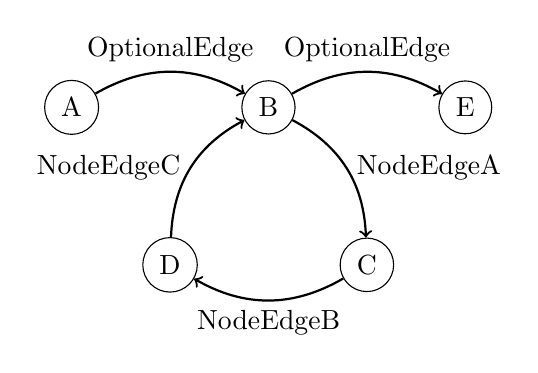
\begin{tikzpicture}
		\tikzset{vertex/.style = {shape=circle,draw,minimum size=.2em}}
		\tikzset{edge/.style = {->,> = latex'}}
		\node[vertex] (a) at  (0,0) {A};
		\node[vertex] (b) at  (2.5,0) {B};
		\node[vertex] (c) at  (3.75,-2) {C};
		\node[vertex] (d) at  (1.25,-2) {D};
		\node[vertex] (e) at  (5,0) {E};
		\path[->,draw,thick, bend left] (a) edge node[above] {OptionalEdge} (b);
		\path[->,draw,thick, bend left] (b) edge node[above] {OptionalEdge} (e);
		\path[->,draw,thick, bend left] (b) edge node[right] {NodeEdgeA} (c);
		\path[->,draw,thick, bend left] (c) edge node[below] {NodeEdgeB} (d);
		\path[->,draw,thick, bend left] (d) edge node[left] {NodeEdgeC} (b);
	\end{tikzpicture}
    \caption{Diagramm einer Sequenz innerhalb eines Schleifen-Knotens}
    \label{FIG:DiagramSequenceInLoop}
  \end{subfigure}
  \begin{subfigure}[c]{0.49\textwidth}
    \lstinputlisting[language=Java,caption={Java-Interface aus einer Sequenz in einem Schleifen-Knoten},label={LST:JInterfaceSequenceInLoop}]{Sequence_in_loop.java}
  \end{subfigure}
  \caption{Diagramm und Interface einer Sequenz innerhalb eines Schleifen-Knotens (nach Variante 2) (\texttt{<rule> = \{NodeEdgeA NodeEdgeB NodeEdgeC\};})}
  \label{FIG:SequenceInLoop}
\end{figure}

\subsubsection{Alternative in einer Schleife}
Befindet sich eine Alternative in einer Schleife, werden alle Alternativen, die nur aus einer Kante bestehen, in eine Schleifen-Kante am Ziel-Knoten der Schleife transformiert. Besteht eine Alternative aus einer Sequenz, wird aus dieser Sequenz eine weitere Schleife aus mehreren Kanten und Knoten (siehe Abbildung~\ref{FIG:DiagramAlternativeInLoop}).

Falls die Alternative sich in einer Sequenz in einer Alternative befindet, gibt es in der Schleife mehrere ausgehende Kanten vom Ziel-Knoten der Schleife.
\begin{figure}[ht]
\centering
  \begin{subfigure}[c]{0.49\textwidth}
  	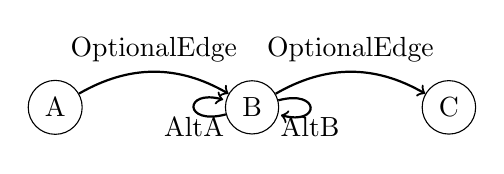
\begin{tikzpicture}
		\tikzset{vertex/.style = {shape=circle,draw,minimum size=.2em}}
		\tikzset{edge/.style = {->,> = latex'}}
		\node[vertex] (a) at  (0,0) {A};
		\node[vertex] (b) at  (2.5,0) {B};
		\node[vertex] (c) at  (5,0) {C};
		\path[->,draw,thick, bend left] (a) edge node[above] {OptionalEdge} (b);
		\path[->,draw,thick, bend left] (b) edge node[above] {OptionalEdge} (c);
		\path[->,draw,thick, loop left] (b) edge node[below] {AltA} (b);
		\path[->,draw,thick, loop right] (b) edge node[below] {AltB} (b);
	\end{tikzpicture}
    \caption{Diagramm einer Alternative innerhalb eines Schleifen-Knotens}
    \label{FIG:DiagramAlternativeInLoop}
  \end{subfigure}
  \begin{subfigure}[c]{0.49\textwidth}
    \lstinputlisting[language=Java,caption={Java-Interfaces aus einer Alternative in einer Schleife},label={LST:JInterfaceAlternativeInLoop}]{Loop_with_inner_alternative.java}
  \end{subfigure}
  \caption{Diagramm und Interface einer Alternative innerhalb eines Schleifen-Knotens (nach Variante 2) (\texttt{<rule> = \{(AlternativeA | AlternativeB)\};})}
  \label{FIG:AlternativeInLoop}
\end{figure}

\subsubsection{Schleife in Alternative}
Befindet sich eine Schleife in einer Alternative, muss für ihre Kante ein Hilfsknoten eingeführt werden, auch wenn die Schleife nur eine Kante beinhaltet (Knoten C in Abbildung~\ref{FIG:DiagramLoopInAlternative}). Würde man die optionalen Kante direkt von A nach B aufnehmen, wären NodeEdgeB und NodeEdgeC ebenfalls optional und würde nicht dem EBNF-Konstrukt entsprechen.
\begin{figure}[ht]
\centering
  \begin{subfigure}[c]{0.49\textwidth}
  	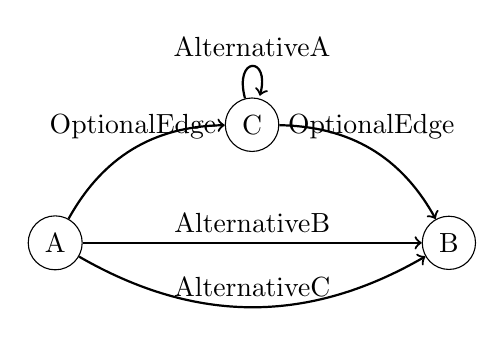
\begin{tikzpicture}
		\tikzset{vertex/.style = {shape=circle,draw,minimum size=.2em}}
		\tikzset{edge/.style = {->,> = latex'}}
		\node[vertex] (a) at  (0,0) {A};
		\node[vertex] (b) at  (5,0) {B};
		\node[vertex] (c) at  (2.5,1.5) {C};
		\path[->,draw,thick, bend left] (a) edge node[above] {OptionalEdge} (c);
		\path[->,draw,thick, loop above] (c) edge node[above] {AlternativeA} (c);
		\path[->,draw,thick, bend left] (c) edge node[above] {OptionalEdge} (b);
		\path[->,draw,thick] (a) edge node[above] {AlternativeB} (b);
		\path[->,draw,thick, bend right] (a) edge node[above] {AlternativeC} (b);
	\end{tikzpicture}
    \caption{Diagramm einer Schleife innerhalb einer Alternative}
    \label{FIG:DiagramLoopInAlternative}
  \end{subfigure}
  \begin{subfigure}[c]{0.49\textwidth}
    \lstinputlisting[language=Java,caption={Java-Interface aus einer Schleife innerhalb einer Alternative},label={LST:JInterfaceLoopInAlternative}]{Alternative_with_inner_loop.java}
  \end{subfigure}
  \caption{Diagramm und Interface einer Schleife innerhalb einer Alternative (\texttt{<rule> = \{NodeEdgeA\} | NodeEdgeB | NodeEdgeC;})}
  \label{FIG:LoopInAlternative}
\end{figure}

\subsection{Scala}
Da es in Scala keine Interfaces gibt, kommen entweder abstrakte Klassen oder Traits infrage. Da Schleifen in einer Alternative Mehrfachvererbung voraussetzen, scheiden die abstrakten Klassen aus.

Es werden also Traits generiert, die die selben Methoden wie die Interface-Pendants haben und (bis auf void, das auf Unit abgebildet wird) die gleichen Parameter- und Rückgabetypen haben, da die Java-Typen verwendet werden können.

Beispielhaft wird hier noch einmal die optionale Schleife aufgeführt (Abbildung~\ref{FIG:ScalaLoopNodeAlt}), um den generierten Scala-Code zu zeigen, weil bei der Schleife Methoden und Vererbung vorkommen.
\begin{figure}[ht]
\centering
  \begin{subfigure}[c]{0.49\textwidth}
  	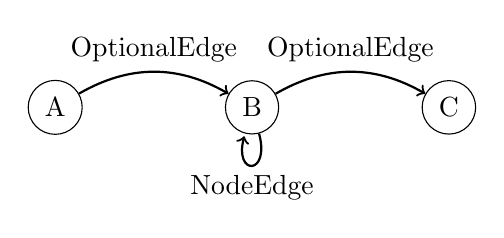
\begin{tikzpicture}
		\tikzset{vertex/.style = {shape=circle,draw,minimum size=.2em}}
		\tikzset{edge/.style = {->,> = latex'}}
		\node[vertex] (a) at  (0,0) {A};
		\node[vertex] (b) at  (2.5,0) {B};
		\node[vertex] (c) at  (5,0) {C};
		\path[->,draw,thick, bend left] (a) edge node[above] {OptionalEdge} (b);
		\path[->,draw,thick, loop below] (b) edge node[below] {NodeEdge} (b);
		\path[->,draw,thick, bend left] (b) edge node[above] {OptionalEdge} (c);
	\end{tikzpicture}
    \caption{Diagramm einer Schleifen-Kante (Variante 2)}
    \label{FIG:ScalaDiagramLoopNodeAlt}
  \end{subfigure}
  \begin{subfigure}[c]{0.49\textwidth}
    \lstinputlisting[language=Scala,caption={Scala-Trait aus einer Schleifen-Kante (Variante 2)},label={LST:ScalaTraitLoopNodeAlt}]{Scope_loop_alt.scala}
  \end{subfigure}
  \caption{Diagramm und Interface einer Schleifen-Kante (Variante 2) (\texttt{<rule> = \{NodeEdge\};})}
  \label{FIG:ScalaLoopNodeAlt}
\end{figure}


\section{Generierung der Interfaces}
Die Java-Interfaces und Scala-Traits werden mit StringTemplate generiert, die aus dem ANTLR-Projekt hervorging~\cite{stringtemplate.github} und die von Parr auch vorgeschlagen werden~\cite[S. 313 ff]{Parr.2010}. Zwar gibt es auch andere Template-Engines (z.B. Apache Velocity\footnote{\url{http://velocity.apache.org/}}), aber StringTemplate biete eine bessere Trennung von Daten und Template~\cite{parr2004enforcing}.

Listing~\ref{LST:STJavaInterface} zeigt das Template für Java-Interfaces das ein Interface mit beliebig vielen Super-Interfaces und Methoden erzeugen kann. Das Template für Scala-Traits ist analog aufgebaut, mit dem Unterschied, dass die Reihenfolge der Argumentnamen und -typen unterschiedlich ist und das Interface durch Trait ersetzt wurde.

Um das Template zu instantiieren muss die Template-Datei geladen und eine Instanz eines Templates (per Namen) erstellt werden (Listing~\ref{LST:STInstantiation}, Zeilen 2 und 3); danach können die Argumente des Templates gesetzt werden (Listing~\ref{LST:STJavaInterface} Zeile 1, Listing~\ref{LST:STInstantiation} Zeilen 4-7). Da StringTemplate die Argument per Lazy Evaluation anwendet wird der Text erst beim Aufruf der Render-Methode ersetzt (Listing~\ref{LST:STInstantiation} Zeile 8) und somit Kollisionen mit dem Inhalt der Argumente vermieden.
\begin{lstlisting}[language=,caption={String-Template für ein Java-Interface mit Methoden},label=LST:STJavaInterface]
javaInterface(package,interfaceName,parents,methods) ::= <<
package <package>;

public interface <interfaceName> <if(parents)>extends <parents;separator=", "> <endif> {<methods:{method|<javaMethod(method.returnType,method.name,method.arguments)>}>
}

>>

javaMethod(returnType,name,arguments) ::= <<

    <returnType> <name>(<arguments:{argument|<argument.type> <argument.name>};separator=", ">);
>>
\end{lstlisting}

\begin{lstlisting}[caption={Instantiierung eines String-Templates},label=LST:STInstantiation]
String renderInterface(final Interface anInterface) {
    final STGroup stGroup = new STGroupFile("java_interface.stg");
    return stGroup.getInstanceOf(javaInterface)
        .add("package", getTargetPackage())
        .add("interfaceName", anInterface.getName())
        .add("methods", anInterface.getMethods())
        .add("parents", anInterface.getParents())
        .render();
}
\end{lstlisting}

\section{Schwierigkeiten beim Bau}
Beim Erstellen des Prototypen traten einige Schwierigkeiten auf. Die größten werden in diesem Abschnitt besprochen: die Behandlung der Rekursion der EBNF-Grammatik und die der Typen.

\subsection{Behandlung der Rekursion}

\subsection{Typen}

\subsubsection{Mapping auf Typen der Hostsprache}
\begin{itemize}
	\item NTs -> Methoden (Einschränungen)
	\item Interfacenamen beliebig
\end{itemize}

\subsection{Nicht-Terminale}
Nicht-Terminale werden durch ihre Entsprechung aus Terminalen ersetzt, danach werden die Terminale durch die folgenden Regeln abgebildet.

\subsection{Scope-Namen}
Die Sopes werden zunächst durch den Graphen selbst erstellt und nummeriert. Diese Namen könnte man beibehalten, da die Bezeichner der Interfaces nicht direkt benutzt werden (bis auf das Start- und End-Interface).

Um trotzdem sprechende Namen zu vergeben, können die Namen der Methoden des Interfaces bestimmt und diese aneinander gehängt werden. Da das zu Kollisionen führen kann, wird in dem Fall der (eindeutige) Name des Scopes aus dem Graphen am Schluss angehängt.

\subsubsection{Generierung von Typen aus EBNF-Regeln}


\section{Einschränkungen bei der Grammatik}
Die EBNF-Grammatik kann nicht beliebig formuliert sein.

\subsection{Startregel}
In der Grammatik muss eine Startregel definiert sein, die nur ein Nicht-Terminal beinhaltet. Daraus wird das erste Interface als Einstiegspunkt generiert.

\subsection{Lexer-Regeln}
Für jede Lexer-Regel sollte es eine entsprechende Parser-Regel geben, die nur die jeweilige Lexer-Regel beinhaltet. Dadurch kann der Listener des Parsers die Typen auch verarbeiten.

Falls eine Regel innerhalb einer anderen vorkommt, ohne ein Trennsymbol zu einer anderen, darf es ebenfalls keine Lexer-Regel sein, um vom Listener erkannt zu werden.


\chapter{Testlauf mit anschaulichem Beispiel}\label{SEC:Example}

\section{Joi}
\begin{figure}[ht]
    \lstinputlisting[language=Java,caption={Joi-EBNF},label={LST:JOIBNF}]{joi.bnf}
\end{figure}
\begin{figure}[ht]
\centering
\resizebox{0.5\linewidth}{!}{\input{\main/10_Pictures/joi.tex}}
\caption{Graph generiert aus der Joi-EBNF}
\label{FIG:JoiGraph}
\end{figure}

\section{Optimierungspotenzial}


\section{Varianten}


\end{document}
